A continuación mostramos los resultados obtenidos de realizar test de las diversas figuras, especificando cual era el código \textit{Dibu} de entrada, el código \textit{SVG} de salida y la imagen generada.

\subsection{\textbf{Figura:} Rectangle}

Código \textit{Dibu} de entrada:

\begin{lstlisting}
  size height=400, width= 1200
  rectangle size=(398, 1198), upper_left=(1,1), fill="none", stroke="blue", stroke-width=2
  rectangle upper_left=(400,100), fill="yellow", size=(200, 400), stroke-width=10, stroke="navy"
\end{lstlisting}

Código \textit{SVG} de salida:

\begin{lstlisting}
  <?xml version="1.0"?>
  <svg height="400" width="1200" >
   <g style="fill-opacity:1.0; stroke:black;
    stroke-width:1;">
    <rect x="1" y="1" height="398"
      width="1198" style="fill:none;stroke:blue;stroke-width:2" />
    <rect x="400" y="100" height="200"
      width="400" style="fill:yellow;stroke:navy;stroke-width:10" />
   </g>
  </svg>
\end{lstlisting}

\begin{figure}[H]
\centering

\includegraphics[width=150mm]{imagenes/rectangle.jpg}
\caption{Imagen generada - Figura Rectangle}
\end{figure}

\subsection{\textbf{Figura:} Line}

Código \textit{Dibu} de entrada:

\begin{lstlisting}
  size width=1200, height=400
  rectangle size=(398, 1198), upper_left=(1,1), fill="none", stroke="blue", stroke-width=2
  line from=(100,300), to=(300,100), stroke-width=5, stroke="green"
  line from=(300,300), to=(500,100), stroke-width=10, stroke="green"
  line from=(500,300), to=(700,100), stroke-width=15, stroke="green"
  line from=(700,300), to=(900,100), stroke-width=20, stroke="green"
  line from=(900,300), to=(1100,100), stroke-width=25, stroke="green"
\end{lstlisting}

Código \textit{SVG} de salida:

\begin{lstlisting}
  <?xml version="1.0"?>
  <svg height="400" width="1200" >
   <g style="fill-opacity:1.0; stroke:black;
    stroke-width:1;">
    <rect x="1" y="1" height="398"
      width="1198" style="fill:none;stroke:blue;stroke-width:2" />
    <line x1="100" y1="300" x2="300" y2="100" style="fill:black;stroke:green;stroke-width:5"/>
    <line x1="300" y1="300" x2="500" y2="100" style="fill:black;stroke:green;stroke-width:10"/>
    <line x1="500" y1="300" x2="700" y2="100" style="fill:black;stroke:green;stroke-width:15"/>
    <line x1="700" y1="300" x2="900" y2="100" style="fill:black;stroke:green;stroke-width:20"/>
    <line x1="900" y1="300" x2="1100" y2="100" style="fill:black;stroke:green;stroke-width:25"/>
   </g>
  </svg>
\end{lstlisting}


\begin{figure}[H]
\centering

\includegraphics[width=150mm]{imagenes/line.jpg}
\caption{Imagen generada - Figura Linea}
\end{figure}

\subsection{\textbf{Figura:} Circle}

Código \textit{Dibu} de entrada:

\begin{lstlisting}
  size width=1200, height=400
  rectangle size=(398, 1198), upper_left=(1,1), fill="none", stroke="blue", stroke-width=2
  circle center=(600, 200), fill="red", stroke="blue", stroke-width=10, radius=100
\end{lstlisting}

Código \textit{SVG} de salida:

\begin{lstlisting}
  <?xml version="1.0"?>
  <svg height="400" width="1200" >
   <g style="fill-opacity:1.0; stroke:black;
    stroke-width:1;">
    <rect x="1" y="1" height="398"
      width="1198" style="fill:none;stroke:blue;stroke-width:2" />
    <circle cx="600" cy="200" r="100"
      style="fill:red;stroke:blue;stroke-width:10"  />
   </g>
  </svg>
\end{lstlisting}

\begin{figure}[H]
\centering

\includegraphics[width=150mm]{imagenes/circle.jpg}
\caption{Imagen generada - Figura Circulo}
\end{figure}

\subsection{\textbf{Figura:} Ellipse}

Código \textit{Dibu} de entrada:

\begin{lstlisting}
  size width=1200, height=400
  rectangle size=(398, 1198), upper_left=(1,1), fill="none", stroke="blue", stroke-width=2
  ellipse center=(300, 200), fill="red", ry=100, rx=250
  ellipse ry=100, fill="none", rx=250, center=(900, 200), stroke="blue", stroke-width=20
\end{lstlisting}

Código \textit{SVG} de salida:

\begin{lstlisting}
  <?xml version="1.0"?>
  <svg height="400" width="1200" >
   <g style="fill-opacity:1.0; stroke:black;
    stroke-width:1;">
    <rect x="1" y="1" height="398"
      width="1198" style="fill:none;stroke:blue;stroke-width:2" />
    <ellipse cx="300" cy="200" rx="250" ry="100"
      style="fill:red;stroke:none;stroke-width:1"/>
    <ellipse cx="900" cy="200" rx="250" ry="100"
      style="fill:none;stroke:blue;stroke-width:20"/>
   </g>
  </svg>
\end{lstlisting}

\begin{figure}[H]
\centering
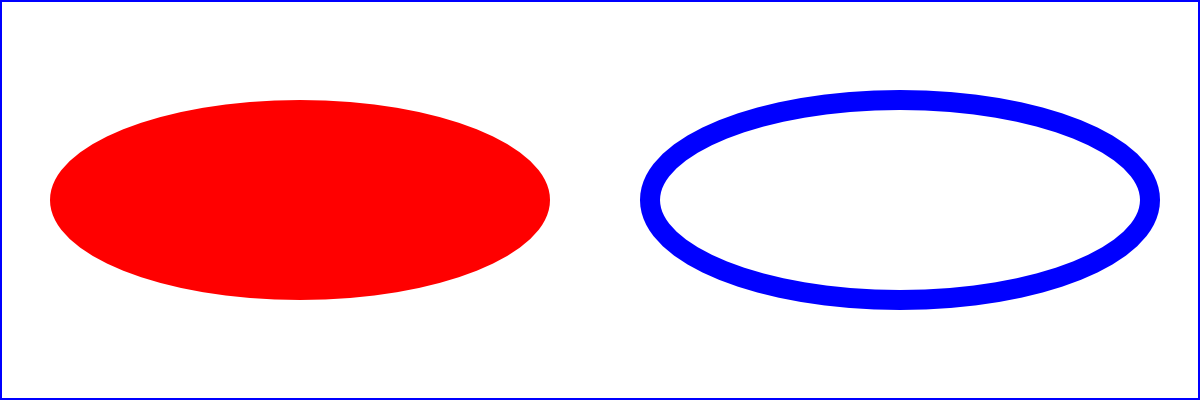
\includegraphics[width=150mm]{imagenes/ellipse.jpg}
\caption{Imagen generada - Figura Elipse}
\end{figure}

\subsection{\textbf{Figura:} Polyline}

Código \textit{Dibu} de entrada:

\begin{lstlisting}
  size width=1200, height=400
  rectangle size=(398, 1198), upper_left=(1,1), fill="none", stroke="blue", stroke-width=2
  polyline points=[(50,375), (150,375), (150,325), (250,325), (250,375), (350,375), (350,250), (450,250), (450,375), (550,375), (550,175), (650,175), (650,375), (750,375), (750,100), (850,100), (850,375), (950,375), (950,25), (1050,25), (1050,375), (1150,375)], stroke="blue", stroke-width=10, fill="none"
\end{lstlisting}

Código \textit{SVG} de salida:

\begin{lstlisting}
  <?xml version="1.0"?>
  <svg height="400" width="1200" >
   <g style="fill-opacity:1.0; stroke:black;
    stroke-width:1;">
    <rect x="1" y="1" height="398"
      width="1198" style="fill:none;stroke:blue;stroke-width:2" />
  <polyline points=" 50,375 150,375 150,325 250,325 250,375 350,375 350,250 450,250 450,375 550,375 550,175 650,175 650,375 750,375 750,100 850,100 850,375 950,375 950,25 1050,25 1050,375 1150,375"
  style="fill:none;stroke:blue;stroke-width:10"/>
   </g>
  </svg>
\end{lstlisting}

\begin{figure}[H]
\centering
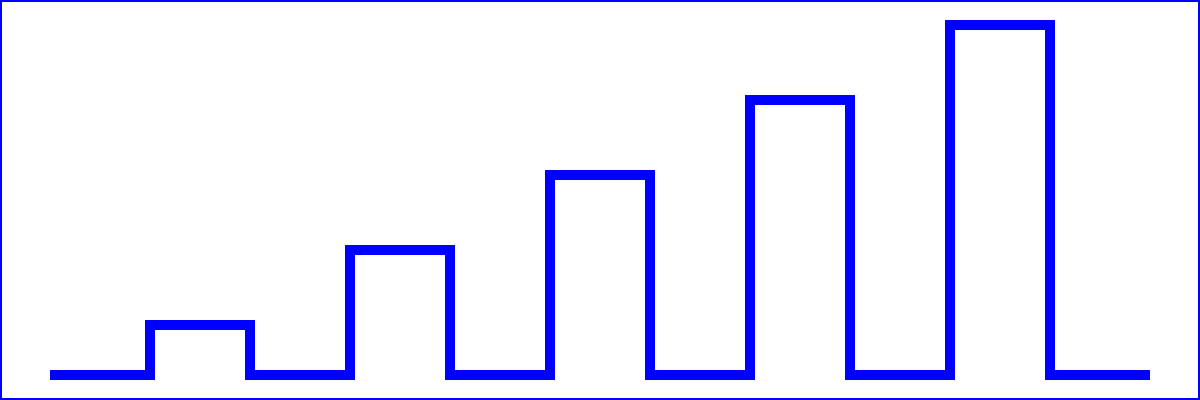
\includegraphics[width=150mm]{imagenes/polyline.jpg}
\caption{Imagen generada - Figura Polyline}
\end{figure}

\subsection{\textbf{Figura:} Polygon}

Código \textit{Dibu} de entrada:

\begin{lstlisting}
  size width=1200, height=400
  rectangle size=(398, 1198), upper_left=(1,1), fill="none", stroke="blue", stroke-width=2
  polygon fill="red", stroke="blue", stroke-width=10, points=[(350,75), (379,161), (469,161), (397,215), (423,301), (350,250), (277,301), (303,215), (231,161), (321,161)]
  polygon fill="lime", stroke="blue", stroke-width=10, points=[(850,75), (958,137.5), (958,262.5), (850,325), (742,262.6), (742,137.5)]
\end{lstlisting}

Código \textit{SVG} de salida:

\begin{lstlisting}
  <?xml version="1.0"?>
  <svg height="400" width="1200" >
   <g style="fill-opacity:1.0; stroke:black;
    stroke-width:1;">
    <rect x="1" y="1" height="398"
      width="1198" style="fill:none;stroke:blue;stroke-width:2" />
  <polygon points=" 350,75 379,161 469,161 397,215 423,301 350,250 277,301 303,215 231,161 321,161"
  style="fill:red;stroke:blue;stroke-width:10"/>
  <polygon points=" 850,75 958,137 958,262 850,325 742,262 742,137"
  style="fill:lime;stroke:blue;stroke-width:10"/>
   </g>
  </svg>
\end{lstlisting}


\begin{figure}[H]
\centering
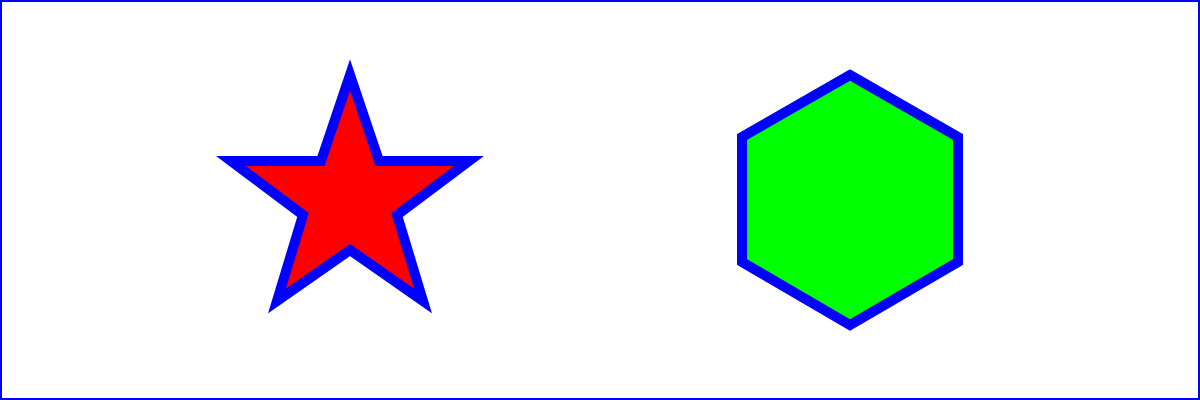
\includegraphics[width=150mm]{imagenes/polygon.jpg}
\caption{Imagen generada - Figura Poligono}
\end{figure}

\newpage

\subsection{Errores Semánticos}
Otra de las cuestiones que nos pareció importante testear es la capacidad del parser de detectar errores semánticos. A partir del enunciado, concluimos que podrían darse los siguientes errores de esta índole:
\begin{enumerate}
  \item \textbf{Dos o mas usos de la sentencia Size.}
  \item \textbf{Nombre de figura invalida.}
  \item \textbf{Parámetro invalido.}
  \item \textbf{Ausencia de parámetros obligatorios.}
  \item \textbf{Parámetros repetidos.}
\end{enumerate}

Propusimos los siguientes test para testear esta característica:
\begin{enumerate}
  \item \textbf{Dos o mas usos de la sentencia Size.}

  Código \textit{Dibu} de entrada:

  \begin{lstlisting}
    size width=1200, height=400
    rectangle upper_left=(1,1), fill="none", stroke="blue", stroke-width=2, size=(200, 200)
    size height=400, width=200
    size height=800, width=800
    rectangle upper_left=(50,50), fill="none", stroke="red", stroke-width=2, size=(500, 800)
  \end{lstlisting}

  Texto emitido en el stdout:

  \begin{lstlisting}
    Semantic error: Dos o Mas Size
    line: 3
    position: 116
  \end{lstlisting}

  \item \textbf{Nombre de figura invalida.}

  Código \textit{Dibu} de entrada:

  \begin{lstlisting}
    cuadrado size=200, fill="red"
    rectangle upper_left=(1,1), fill="none", stroke="blue", stroke-width=2, size=(200, 200)
  \end{lstlisting}

  Texto emitido en el stdout:

  \begin{lstlisting}
    Semantic error: Figura Invalida
    line: 1
    position: 9
  \end{lstlisting}

  \item \textbf{Parámetro invalido.}

  Código \textit{Dibu} de entrada:

  \begin{lstlisting}
    line from=(100,300), to=(300,100), stroke-width=5, stroke="green"
    line from=(300,300), to=(500,100), stroke-width=10, stroke="green", rotate=(90,90)
  \end{lstlisting}

  Texto emitido en el stdout:

  \begin{lstlisting}
    Semantic error: Parametro Invalido
    line: 2
    position: 71
  \end{lstlisting}

  \item \textbf{Ausencia de parámetros obligatorios.}

  Código \textit{Dibu} de entrada:

  \begin{lstlisting}
    line to=(300,100), stroke-width=5, stroke="green"
    line from=(300,300), to=(500,100), stroke-width=10, stroke="green"
  \end{lstlisting}

  Texto emitido en el stdout:

  \begin{lstlisting}
    Semantic error: Faltan Parametros obligatorios
    line: 1
    position: 5
  \end{lstlisting}

  \item \textbf{Parámetros repetidos.}

  Código \textit{Dibu} de entrada:

  \begin{lstlisting}
    line from=(100,100), to=(300,100), stroke-width=5, stroke="green", stroke-width=3
    line from=(300,300), to=(500,100), stroke-width=10, stroke="green"
  \end{lstlisting}

  Texto emitido en el stdout:

  \begin{lstlisting}
    Semantic error: Parametros repetidos
    line: 1
    position: 35
  \end{lstlisting}

\end{enumerate}
